% Use apenas no projeto (TCC I). Remova o \input correspondente na monografia final.
\chapter{Cronograma}\label{sec:cronograma}

\begin{dica}[Dica de metodologia científica: cronograma]
O cronograma mostra que o trabalho é viável: liste as atividades na ordem lógica
(revisão bibliográfica, levantamento de requisitos, modelagem, implementação, testes,
escrita, defesa), com duração realista e margem para imprevistos, e relacione-as aos
objetivos específicos. Em \ac{tcc} I (projeto), o cronograma é elemento esperado; na
monografia final, em geral, é suprimido. Como o cronograma não traz dados numéricos,
ele é um \textbf{quadro} (e não uma tabela); diagramas (Gantt e PERT/CPM) são
\textbf{figuras}.
\end{dica}

\begin{dica}[Dica de uso da classe: quatro formas de apresentar o cronograma]
Escolha \emph{uma} das formas abaixo. As duas primeiras são quadros (\texttt{quadro} com
\texttt{ilustracao}): marcas nos meses e células sombreadas (pacote \texttt{colortbl}), que
imprime bem em preto e branco. As duas últimas são figuras desenhadas com TikZ: o diagrama
de Gantt (desenhado em TikZ) mostra as atividades como barras ao longo do tempo, e
o diagrama PERT/CPM mostra as \emph{dependências} entre as atividades, as folgas e o caminho
crítico, sendo o mais adequado quando a ordem de execução importa. Em todos os exemplos o
objeto ocupa a largura do texto sem alterar o tamanho da letra: o primeiro e o segundo usam
\texttt{tabularx} com uma coluna \texttt{X} elástica; o terceiro calcula a unidade horizontal
a partir de \texttt{\textbackslash linewidth}; o quarto distribui os nós na largura. Em
qualquer caso a fonte é obrigatória e a legenda explica o símbolo usado.
\end{dica}

\section{Opção A: quadro com marcas}

O cronograma das atividades é apresentado no \autoref{qua:cronograma}.

\begin{quadro}[htbp]
\begin{ilustracao}[\linewidth]{\caption{Cronograma do projeto em meses}\label{qua:cronograma}}{\elaboracaopropria\legenda{O símbolo $\bullet$ indica o mês em que a atividade é executada.}}
  \small
  \begin{tabularx}{\linewidth}{|l|*{12}{>{\centering\arraybackslash}X|}}
    \hline
    \textbf{Atividade} & \textbf{1} & \textbf{2} & \textbf{3} & \textbf{4} & \textbf{5} & \textbf{6} & \textbf{7} & \textbf{8} & \textbf{9} & \textbf{10} & \textbf{11} & \textbf{12} \\
    \hline
    Revisão bibliográfica & $\bullet$ & $\bullet$ & & & & & & & & & & \\
    \hline
    Métodos & & & $\bullet$ & $\bullet$ & & & & & & & & \\
    \hline
    Testes & & & & $\bullet$ & $\bullet$ & $\bullet$ & & & & & & \\
    \hline
    Resultados & & & & & & & $\bullet$ & $\bullet$ & & & & \\
    \hline
    Conclusão & & & & & & & $\bullet$ & $\bullet$ & $\bullet$ & & & \\
    \hline
    Banca & & & & & & & & & & $\bullet$ & $\bullet$ & $\bullet$ \\
    \hline
  \end{tabularx}
\end{ilustracao}
\end{quadro}

\section{Opção B: quadro com células sombreadas}

O \autoref{qua:cronograma-cor} traz o mesmo cronograma com as células do período
sombreadas, com o cabeçalho ``Mês'' agrupando as doze colunas e linhas mais altas para
melhorar a leitura.

\newcommand{\mes}{\cellcolor{black!35}}

\begin{quadro}[htbp]
\begin{ilustracao}[\linewidth]{\caption{Cronograma do projeto com células sombreadas}\label{qua:cronograma-cor}}{\elaboracaopropria\legenda{As células sombreadas indicam os meses de execução de cada atividade.}}
  \small
  \renewcommand{\arraystretch}{1.5}
  \begin{tabularx}{\linewidth}{|l|*{12}{>{\centering\arraybackslash}X|}}
    \hline
    \multirow{2}{*}{\textbf{Atividade}} & \multicolumn{12}{c|}{\textbf{Mês}} \\
    \cline{2-13}
     & 1 & 2 & 3 & 4 & 5 & 6 & 7 & 8 & 9 & 10 & 11 & 12 \\
    \hline
    Revisão bibliográfica & \mes & \mes & & & & & & & & & & \\
    \hline
    Métodos & & & \mes & \mes & & & & & & & & \\
    \hline
    Testes & & & & \mes & \mes & \mes & & & & & & \\
    \hline
    Resultados & & & & & & & \mes & \mes & & & & \\
    \hline
    Conclusão & & & & & & & \mes & \mes & \mes & & & \\
    \hline
    Banca & & & & & & & & & & \mes & \mes & \mes \\
    \hline
  \end{tabularx}
\end{ilustracao}
\end{quadro}

\section{Opção C: diagrama de Gantt}

A \autoref{fig:gantt} apresenta o cronograma como um diagrama de Gantt, que mostra as
atividades como barras ao longo do tempo e deixa evidentes as sobreposições. Ele é
desenhado diretamente em TikZ, em uma grade única: os nomes das atividades ficam
\emph{dentro} da moldura, em uma primeira coluna, e o diagrama ocupa toda a largura do
texto (a largura de cada mês é calculada a partir de \texttt{\textbackslash linewidth}).
Para mudar as atividades, edite a lista do \texttt{\textbackslash foreach} no formato
\texttt{nome/mês inicial/mês final} e ajuste \texttt{\textbackslash ufvnativ} (número de
atividades).

\begin{figure}[htbp]
\begin{ilustracao}[\linewidth]{\caption{Diagrama de Gantt do cronograma do projeto}\label{fig:gantt}}{\elaboracaopropria\legenda{Cada barra indica a duração da atividade, em meses.}}
  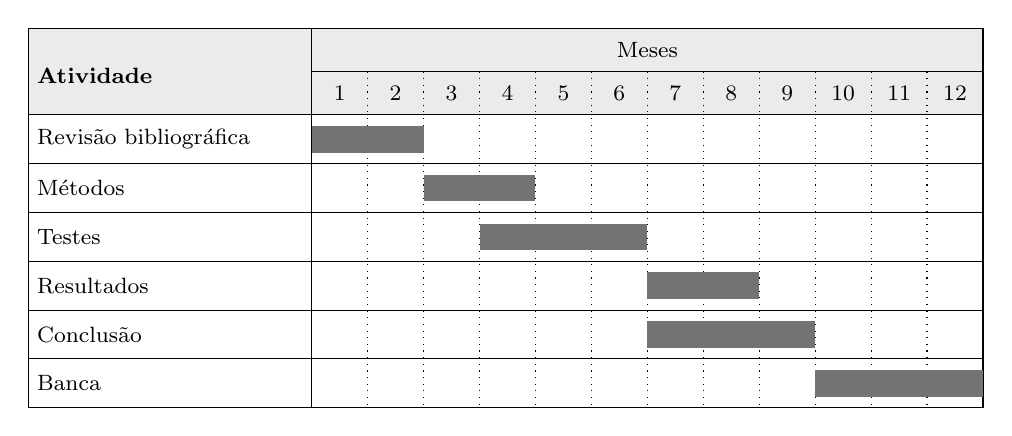
\begin{tikzpicture}[font=\footnotesize, line width=0.4pt]
    \def\ufvnativ{6}                                      % número de atividades
    \pgfmathsetlengthmacro{\ufvlc}{3.6cm}                 % largura da coluna de atividades
    \pgfmathsetlengthmacro{\ufvxu}{(\linewidth-\ufvlc)/12} % largura de cada mês
    \pgfmathsetlengthmacro{\ufvhh}{1.1cm}                 % altura do cabeçalho (2 linhas)
    \pgfmathsetlengthmacro{\ufvrh}{0.62cm}                % altura de cada atividade
    \pgfmathsetlengthmacro{\ufvht}{\ufvhh+\ufvnativ*\ufvrh} % altura total
    % cabeçalho sombreado, moldura e linhas
    \fill[black!8] (0,0) rectangle (\linewidth,-\ufvhh);
    \draw (0,0) rectangle (\linewidth,-\ufvht);
    \draw (0,-\ufvhh) -- (\linewidth,-\ufvhh);
    \draw (\ufvlc,0) -- (\ufvlc,-\ufvht);
    \draw (\ufvlc,-0.55cm) -- (\linewidth,-0.55cm);
    \node[anchor=west, inner xsep=3pt, font=\footnotesize\bfseries] at (0,-0.55*\ufvhh) {Atividade};
    \node at ({\ufvlc+6*\ufvxu},-0.275cm) {Meses};
    \foreach \m in {1,...,12} {
      \node at ({\ufvlc+(\m-0.5)*\ufvxu},-0.825cm) {\m};
      \draw[dotted] ({\ufvlc+\m*\ufvxu},-0.55cm) -- ({\ufvlc+\m*\ufvxu},-\ufvht);
    }
    % atividades: nome/mês inicial/mês final
    \foreach \nome/\ini/\fim [count=\k] in {Revisão bibliográfica/1/2, Métodos/3/4,
        Testes/4/6, Resultados/7/8, Conclusão/7/9, Banca/10/12} {
      \pgfmathsetlengthmacro{\yt}{-\ufvhh-(\k-1)*\ufvrh}
      \draw (0,\yt) -- (\linewidth,\yt);
      \node[anchor=west, inner xsep=3pt] at (0,\yt-0.5*\ufvrh) {\nome};
      \fill[black!55] ({\ufvlc+(\ini-1)*\ufvxu},\yt-0.14cm) rectangle ({\ufvlc+\fim*\ufvxu},\yt-\ufvrh+0.14cm);
    }
  \end{tikzpicture}
\end{ilustracao}
\end{figure}
